\documentclass[11pt,a4paper]{article}

% Pacotes essenciais
\usepackage[utf8]{inputenc}
\usepackage[T1]{fontenc}
\usepackage{lmodern}
\usepackage[portuguese]{babel}
\usepackage{graphicx}
\usepackage{amsmath}
\usepackage{amsfonts}
\usepackage{amssymb}
\usepackage{float}
\usepackage{caption}
\usepackage{subcaption}
\usepackage{xcolor}
\usepackage{fancyhdr}
\usepackage{geometry}
\usepackage{titlesec}
\usepackage{lipsum}
\usepackage{cite}
\usepackage{booktabs}
\usepackage{array}
\usepackage{tikz}
\usepackage[hidelinks]{hyperref}

% Definição das cores
\definecolor{headercolor}{HTML}{b11116}
\definecolor{secondarycolor}{HTML}{3a5461}

% Configuração da página
\geometry{
    a4paper,
    top=2.8cm,
    bottom=2.5cm,
    left=2.5cm,
    right=2.5cm,
    headheight=1.2cm,
    headsep=0.5cm
}

% Configuração do cabeçalho
\pagestyle{fancy}
\fancyhf{}
\renewcommand{\headrulewidth}{0pt}
\renewcommand{\footrulewidth}{0.5pt}

\fancyhead[L]{%
    \begin{tikzpicture}[remember picture, overlay]
        \fill[headercolor] (current page.north west) rectangle ([yshift=-1.2cm]current page.north east);
        \node[anchor=west, inner sep=0pt] at ([xshift=1cm, yshift=-0.6cm]current page.north west) 
            {
\includegraphics[height=0.8cm]{imgs/base/fatec-rgt.png}};
        \node[anchor=east, inner sep=0pt] at ([xshift=-1cm, yshift=-0.6cm]current page.north east) 
            {
\includegraphics[height=0.9cm]{imgs/base/cps-logo.png}};
        \node[anchor=east, inner sep=0pt] at ([xshift=-2.8cm, yshift=-0.6cm]current page.north east) 
            {
\includegraphics[height=1.05cm]{imgs/base/governo-sp-secretaria-logo.png}};
    \end{tikzpicture}
}

\fancyfoot[L]{\footnotesize\textcolor{secondarycolor}{Faculdade de Tecnologia do Estado de São Paulo\\ fatecregistro.cps.sp.gov.br}}
\fancyfoot[R]{\thepage}

% Configuração dos títulos das seções
\titleformat{\section}
    {\normalfont\large\bfseries\color{secondarycolor}}
    {\thesection}{1em}{}

\titleformat{\subsection}
    {\normalfont\normalsize\bfseries\color{secondarycolor}}
    {\thesubsection}{1em}{}

% Informações do artigo
\title{
Sistema Educacional de Baixo Custo com Realidade Aumentada para o Ensino Prático de Montagem de Hardware e Redes
}

\author{
Éric Leandro$^{1}$, Lucas Miura$^{1}$, Luiz Medina$^{1}$, Pedro Silva$^{1}$\\[0.3cm]
\small $^{1}$Faculdade de Tecnologia do Estado de São Paulo\\[0.2cm]
\small eric.leandro@aluno.cps.sp.gov.br\\
\small lucas.miura@aluno.cps.sp.gov.br\\
\small luiz.medina@aluno.cps.sp.gov.br\\
\small pedro.silva13@aluno.cps.sp.gov.br
}

\date{}

\begin{document}

% Força o cabeçalho em todas as páginas
\pagestyle{fancy}

\maketitle
\thispagestyle{fancy}

% Resumo
\section*{Resumo}

Este trabalho apresenta o SAVIT, um sistema educacional de baixo custo baseado em Realidade Aumentada (RA), voltado ao ensino prático de montagem de hardware e redes de computadores. A proposta busca oferecer uma experiência interativa e acessível por meio de dispositivos móveis, permitindo que estudantes realizem atividades práticas sem a necessidade de laboratórios físicos ou equipamentos de alto custo. O sistema utiliza Unity, ARCore, MediaPipe e visão computacional para possibilitar a interação com componentes virtuais através de gestos capturados pela câmera do celular. Além disso, a aplicação permite posicionar peças em superfícies reais utilizando Realidade Aumentada, promovendo uma experiência de aprendizado mais intuitiva, dinâmica e imersiva. O projeto busca democratizar o acesso ao ensino técnico, contribuindo para uma aprendizagem mais moderna, acessível e alinhada às tecnologias emergentes.

\vspace{0.3cm}
\noindent\textit{\textbf{Palavras-chave:}} Sistema Educacional; Realidade Aumentada; Visão Computacional; Redes de Computadores.

\vspace{0.5cm}
\noindent\rule{\textwidth}{0.5pt}
\vspace{0.5cm}


% Abstract
\section*{Abstract}

This work presents SAVIT, a low-cost educational system based on Augmented Reality (AR), designed for practical teaching of computer hardware assembly and networking. The proposal aims to provide an interactive and accessible experience through mobile devices, allowing students to perform practical activities without the need for physical laboratories or expensive equipment. The system was developed using Unity, ARCore, MediaPipe, and computer vision techniques to enable interaction with virtual components through gestures captured by the smartphone camera. In addition, the application allows users to place parts on real-world surfaces using Augmented Reality, promoting a more intuitive, dynamic, and immersive learning experience. The project seeks to democratize access to technical education, contributing to a more modern, accessible, and technology-aligned learning process.

\vspace{0.3cm}
\noindent\textit{\textbf{Keywords:}} Educational System; Augmented Reality; Computer Vision; Computer Networks.

\vspace{0.5cm}
\noindent\rule{\textwidth}{0.5pt}
\vspace{0.5cm}


% Introdução
\section{Introdução}

O avanço das tecnologias digitais vem transformando significativamente os métodos de ensino, especialmente em áreas técnicas que exigem atividades práticas, como infraestrutura computacional, montagem de hardware e redes de computadores. Entretanto, muitas instituições de ensino ainda enfrentam dificuldades relacionadas à limitação de laboratórios físicos, falta de equipamentos adequados e altos custos de manutenção, comprometendo a experiência prática dos estudantes.

No primeiro semestre de 2025, foi realizada uma pesquisa de campo com cinquenta estudantes de diferentes semestres da FATEC Registro, provenientes de diferentes cidades do Vale do Ribeira. Os resultados reforçaram a problemática investigada: apenas 26\% dos participantes afirmaram sempre possuir acesso adequado a equipamentos para aulas práticas, enquanto 48\% relataram prejuízos totais ou parciais no aprendizado devido à ausência desses recursos. Além disso, 71\% consideraram que tecnologias acessíveis baseadas em Realidade Aumentada ou Realidade Virtual poderiam contribuir para reduzir as dificuldades decorrentes da limitação de infraestrutura física.

Nesse contexto, a utilização de tecnologias emergentes, como a Realidade Aumentada (RA), surge como uma alternativa capaz de complementar o processo de aprendizagem de maneira interativa e acessível. Diferentemente da Realidade Virtual, que cria ambientes totalmente digitais, a Realidade Aumentada permite integrar objetos virtuais ao ambiente físico real, proporcionando maior contextualização e acessibilidade ao usuário por meio de dispositivos móveis.

Com base nesse cenário, o presente trabalho apresenta o SAVIT, um sistema educacional baseado em Realidade Aumentada, desenvolvido para dispositivos móveis Android. A aplicação permite que os usuários realizem a simulação interativa de montagem de componentes computacionais utilizando gestos capturados pela câmera do celular, promovendo uma experiência prática e intuitiva sem a necessidade de equipamentos físicos reais.

Além disso, o sistema utiliza recursos como visão computacional, reconhecimento de gestos, MediaPipe e ARCore para possibilitar a interação entre o usuário e os componentes tridimensionais posicionados em superfícies reais. Dessa forma, o projeto busca democratizar o acesso ao aprendizado técnico, oferecendo uma solução de baixo custo voltada ao ensino prático de hardware e redes de computadores.


% Objetivo
\section{Objetivo}

O objetivo do SAVIT é proporcionar aos estudantes um ambiente de aprendizado prático baseado em Realidade Aumentada, permitindo a simulação da montagem de componentes computacionais de forma interativa e acessível. A aplicação foi desenvolvida para dispositivos móveis Android, utilizando a câmera do celular para detectar superfícies reais e posicionar objetos tridimensionais no ambiente físico.

Além disso, o sistema utiliza reconhecimento de gestos para possibilitar a movimentação e interação com as peças virtuais, promovendo uma experiência educacional dinâmica e intuitiva. O projeto busca reduzir a dependência de laboratórios físicos e equipamentos de alto custo, ampliando o acesso ao ensino prático na área de infraestrutura computacional.

Entre os objetivos específicos do projeto, destacam-se:

\begin{itemize}
    \item Desenvolver uma aplicação mobile baseada em Realidade Aumentada para o ensino prático de hardware;
    \item Permitir a interação com componentes tridimensionais através de gestos manuais;
    \item Utilizar visão computacional para reconhecimento e movimentação de peças;
    \item Oferecer uma solução educacional acessível utilizando dispositivos móveis compatíveis com ARCore;
    \item Simular atividades práticas de montagem computacional sem necessidade de equipamentos físicos reais.
\end{itemize}

% Estado da Arte
\section{Estado da Arte}

A Realidade Aumentada (RA) vem sendo utilizada como ferramenta de apoio ao ensino técnico e profissionalizante, especialmente em atividades que envolvem visualização espacial, interação tridimensional e treinamento prático. Estudos apontam que sua utilização pode favorecer o engajamento, a compreensão de conteúdos e a aproximação entre conhecimentos teóricos e situações práticas.

Justimiano et al. \cite{justimiano2021} desenvolveram um sistema de RA voltado ao treinamento de procedimentos de montagem e manutenção de equipamentos. A solução atua como apoio à execução de tarefas técnicas, demonstrando o potencial da tecnologia para atividades práticas guiadas. Entretanto, sua aplicação é direcionada a cenários específicos de manutenção e não contempla o ensino de infraestrutura computacional com interação gestual.

Chiang, Shang e Qiao \cite{chiang2022}, em uma revisão sistemática sobre Realidade Aumentada aplicada à formação profissional, identificaram sua utilização principalmente em treinamento médico, manutenção industrial e atividades de montagem. Os autores destacam resultados positivos relacionados ao desenvolvimento de habilidades práticas, embora apontem a necessidade de aplicações educacionais mais maduras e adaptadas aos diferentes contextos de formação profissional.

Supriyanto et al. \cite{supriyanto2023} analisaram aplicações de RA na educação profissional e observaram benefícios relacionados à compreensão, experiência de aprendizagem e participação dos estudantes. Os resultados reforçam o potencial da tecnologia como complemento ao ensino convencional, especialmente em atividades que exigem experiências práticas.

Além das aplicações educacionais, o MediaPipe \cite{lugaresi2019} fornece recursos de visão computacional capazes de reconhecer e rastrear movimentos das mãos em tempo real. Essa abordagem permite desenvolver formas de interação mais naturais com objetos virtuais, reduzindo a necessidade de dispositivos físicos adicionais.

A Tabela \ref{tab:estado-arte} sintetiza as principais características dos trabalhos analisados e evidencia o diferencial proposto pelo SAVIT.

\begin{table}[H]
\centering
\caption{Comparação entre trabalhos relacionados e o SAVIT}
\label{tab:estado-arte}
\small
\begin{tabular}{|p{3.1cm}|p{3.4cm}|p{3.4cm}|p{3.4cm}|}
\hline
\textbf{Trabalho} & \textbf{Aplicação} & \textbf{Contribuição} & \textbf{Limitação / Diferencial} \\
\hline

Justimiano et al. (2021) &
Montagem e manutenção de equipamentos com RA &
Treinamento técnico guiado e interativo &
Não possui foco específico em infraestrutura computacional com interação gestual \\
\hline

Chiang, Shang e Qiao (2022) &
RA aplicada à formação profissional &
Evidencia benefícios da RA em atividades práticas e treinamento &
Revisão ampla, sem propor uma solução específica para montagem de hardware \\
\hline

Supriyanto et al. (2023) &
RA na educação profissional &
Aponta melhorias na compreensão e experiência de aprendizagem &
Analisa diferentes contextos educacionais sem foco específico em hardware \\
\hline

Lugaresi et al. (2019) &
Reconhecimento de mãos com MediaPipe &
Permite rastreamento e interação gestual em tempo real &
Framework de visão computacional, não uma solução educacional completa \\
\hline

SAVIT &
Montagem de hardware em Realidade Aumentada &
Integra RA, visão computacional e gestos em dispositivos móveis &
Propõe interação prática voltada ao ensino de infraestrutura computacional \\
\hline

\end{tabular}
\end{table}

Nesse contexto, o SAVIT diferencia-se por integrar Realidade Aumentada, visão computacional e reconhecimento de gestos em uma aplicação mobile voltada ao ensino de montagem de hardware. A proposta busca combinar acessibilidade e interação natural em um único ambiente educacional, reduzindo a dependência de equipamentos físicos especializados.

% Metodologia
\section{Metodologia}

O desenvolvimento do SAVIT foi realizado por meio de uma abordagem prática e incremental, dividida em etapas de levantamento de requisitos, pesquisa tecnológica, desenvolvimento e testes da aplicação, conforme apresentado na Figura \ref{fig:metodologia}.

\begin{figure}[H]
    \centering
    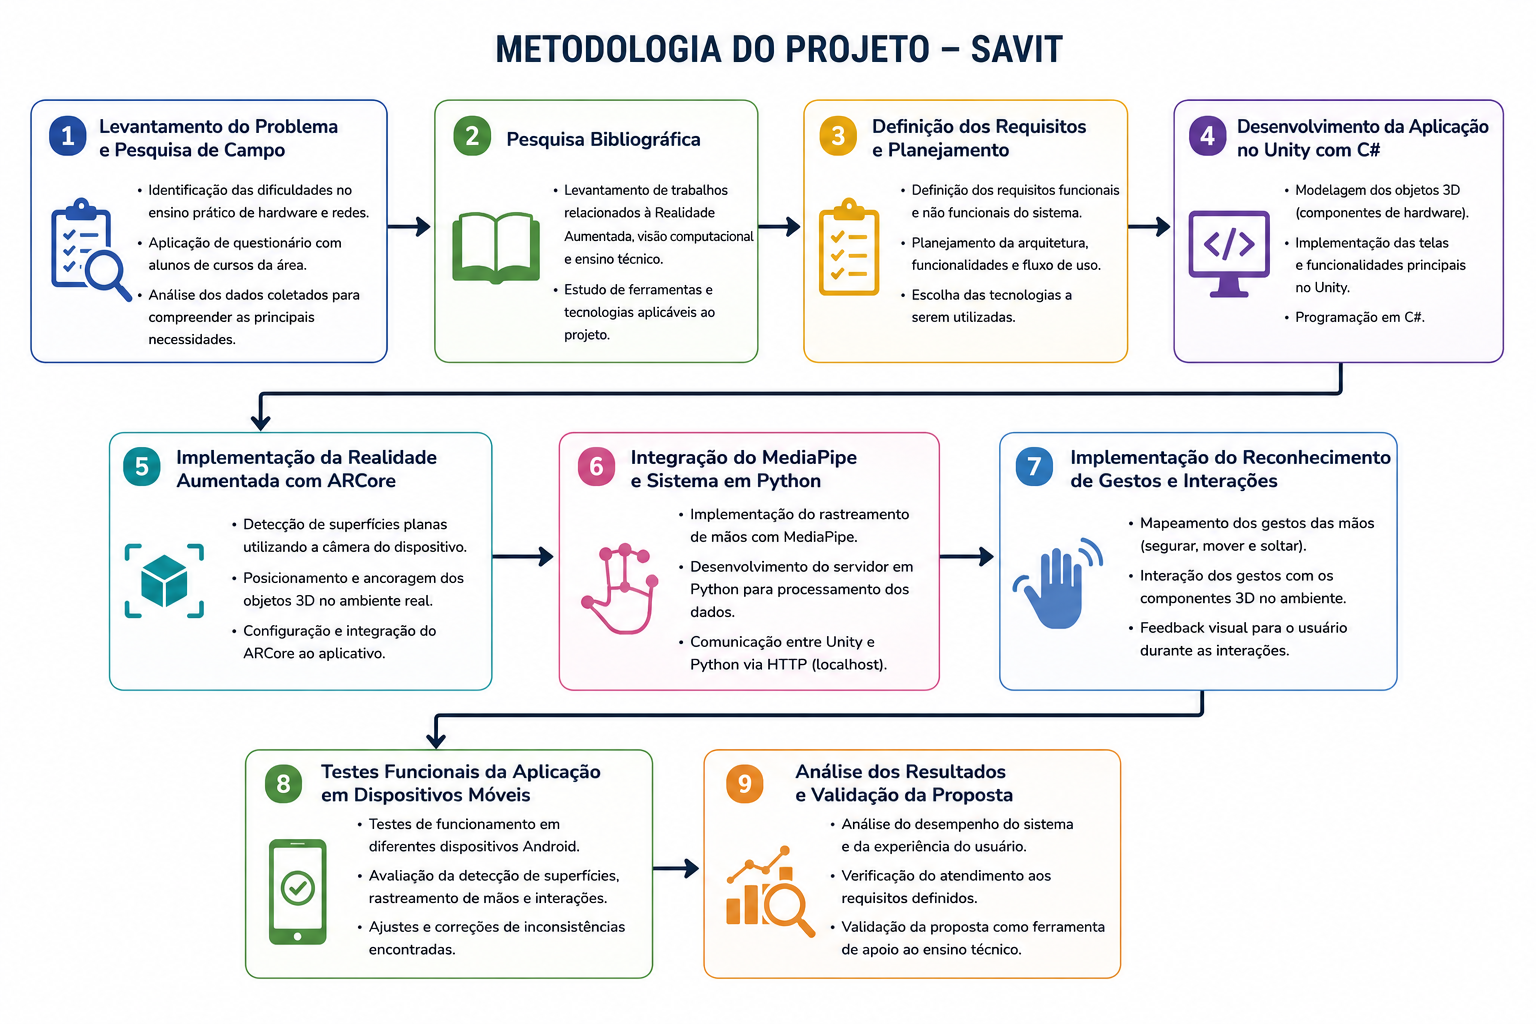
\includegraphics[width=0.85\textwidth]{imgs/metodologia-savit.png}
    \caption{Fluxograma da criação do SAVIT}
    \label{fig:metodologia}
\end{figure}

No primeiro semestre de 2025, foi realizada uma pesquisa de campo presencial com cinquenta estudantes de diferentes semestres da FATEC Registro, provenientes de diferentes cidades do Vale do Ribeira. O questionário, composto por nove perguntas objetivas e discursivas, buscou identificar a disponibilidade de equipamentos para atividades práticas e a percepção dos estudantes sobre os impactos dessa limitação no aprendizado. As respostas discursivas com significados semelhantes foram agrupadas em categorias para posterior tabulação percentual.

Paralelamente, foi realizada uma pesquisa bibliográfica sobre Realidade Aumentada, visão computacional e reconhecimento de gestos aplicados ao contexto educacional. A aplicação foi desenvolvida na Unity utilizando C\#, com AR Foundation e ARCore para detecção de superfícies e posicionamento dos objetos tridimensionais em dispositivos móveis Android. Os componentes utilizados, como memória RAM, placa-mãe e gabinete, foram integrados à aplicação por meio de assets tridimensionais.

A interação com os componentes virtuais utiliza MediaPipe e um sistema complementar desenvolvido em Python para processar os movimentos das mãos capturados pela câmera. A comunicação ocorre por meio de um endpoint HTTP local, permitindo reconhecer gestos para segurar, movimentar e soltar os objetos durante a experiência em Realidade Aumentada.

Por fim, foram realizados testes funcionais e qualitativos relacionados à detecção de superfícies, reconhecimento de gestos, movimentação das peças e estabilidade geral da aplicação, visando verificar o funcionamento do protótipo e sua viabilidade técnica como ferramenta de apoio ao ensino prático de infraestrutura computacional. Nesta etapa, não foram aplicadas métricas quantitativas de desempenho ou de eficácia educacional, constituindo uma limitação a ser considerada em avaliações futuras.

% Resultados e Discussões
\section{Resultados e Discussões}

Os resultados da pesquisa de campo contribuíram para validar a problemática que motivou o desenvolvimento do SAVIT. Conforme apresentado na Figura \ref{fig:pesquisa-q2}, apenas 26\% dos participantes afirmaram possuir sempre acesso adequado aos equipamentos necessários para aulas práticas. Embora 58\% tenham indicado acesso na maioria das vezes, 16\% relataram que raramente ou nunca dispõem desses recursos.

\begin{figure}[H]
    \centering
    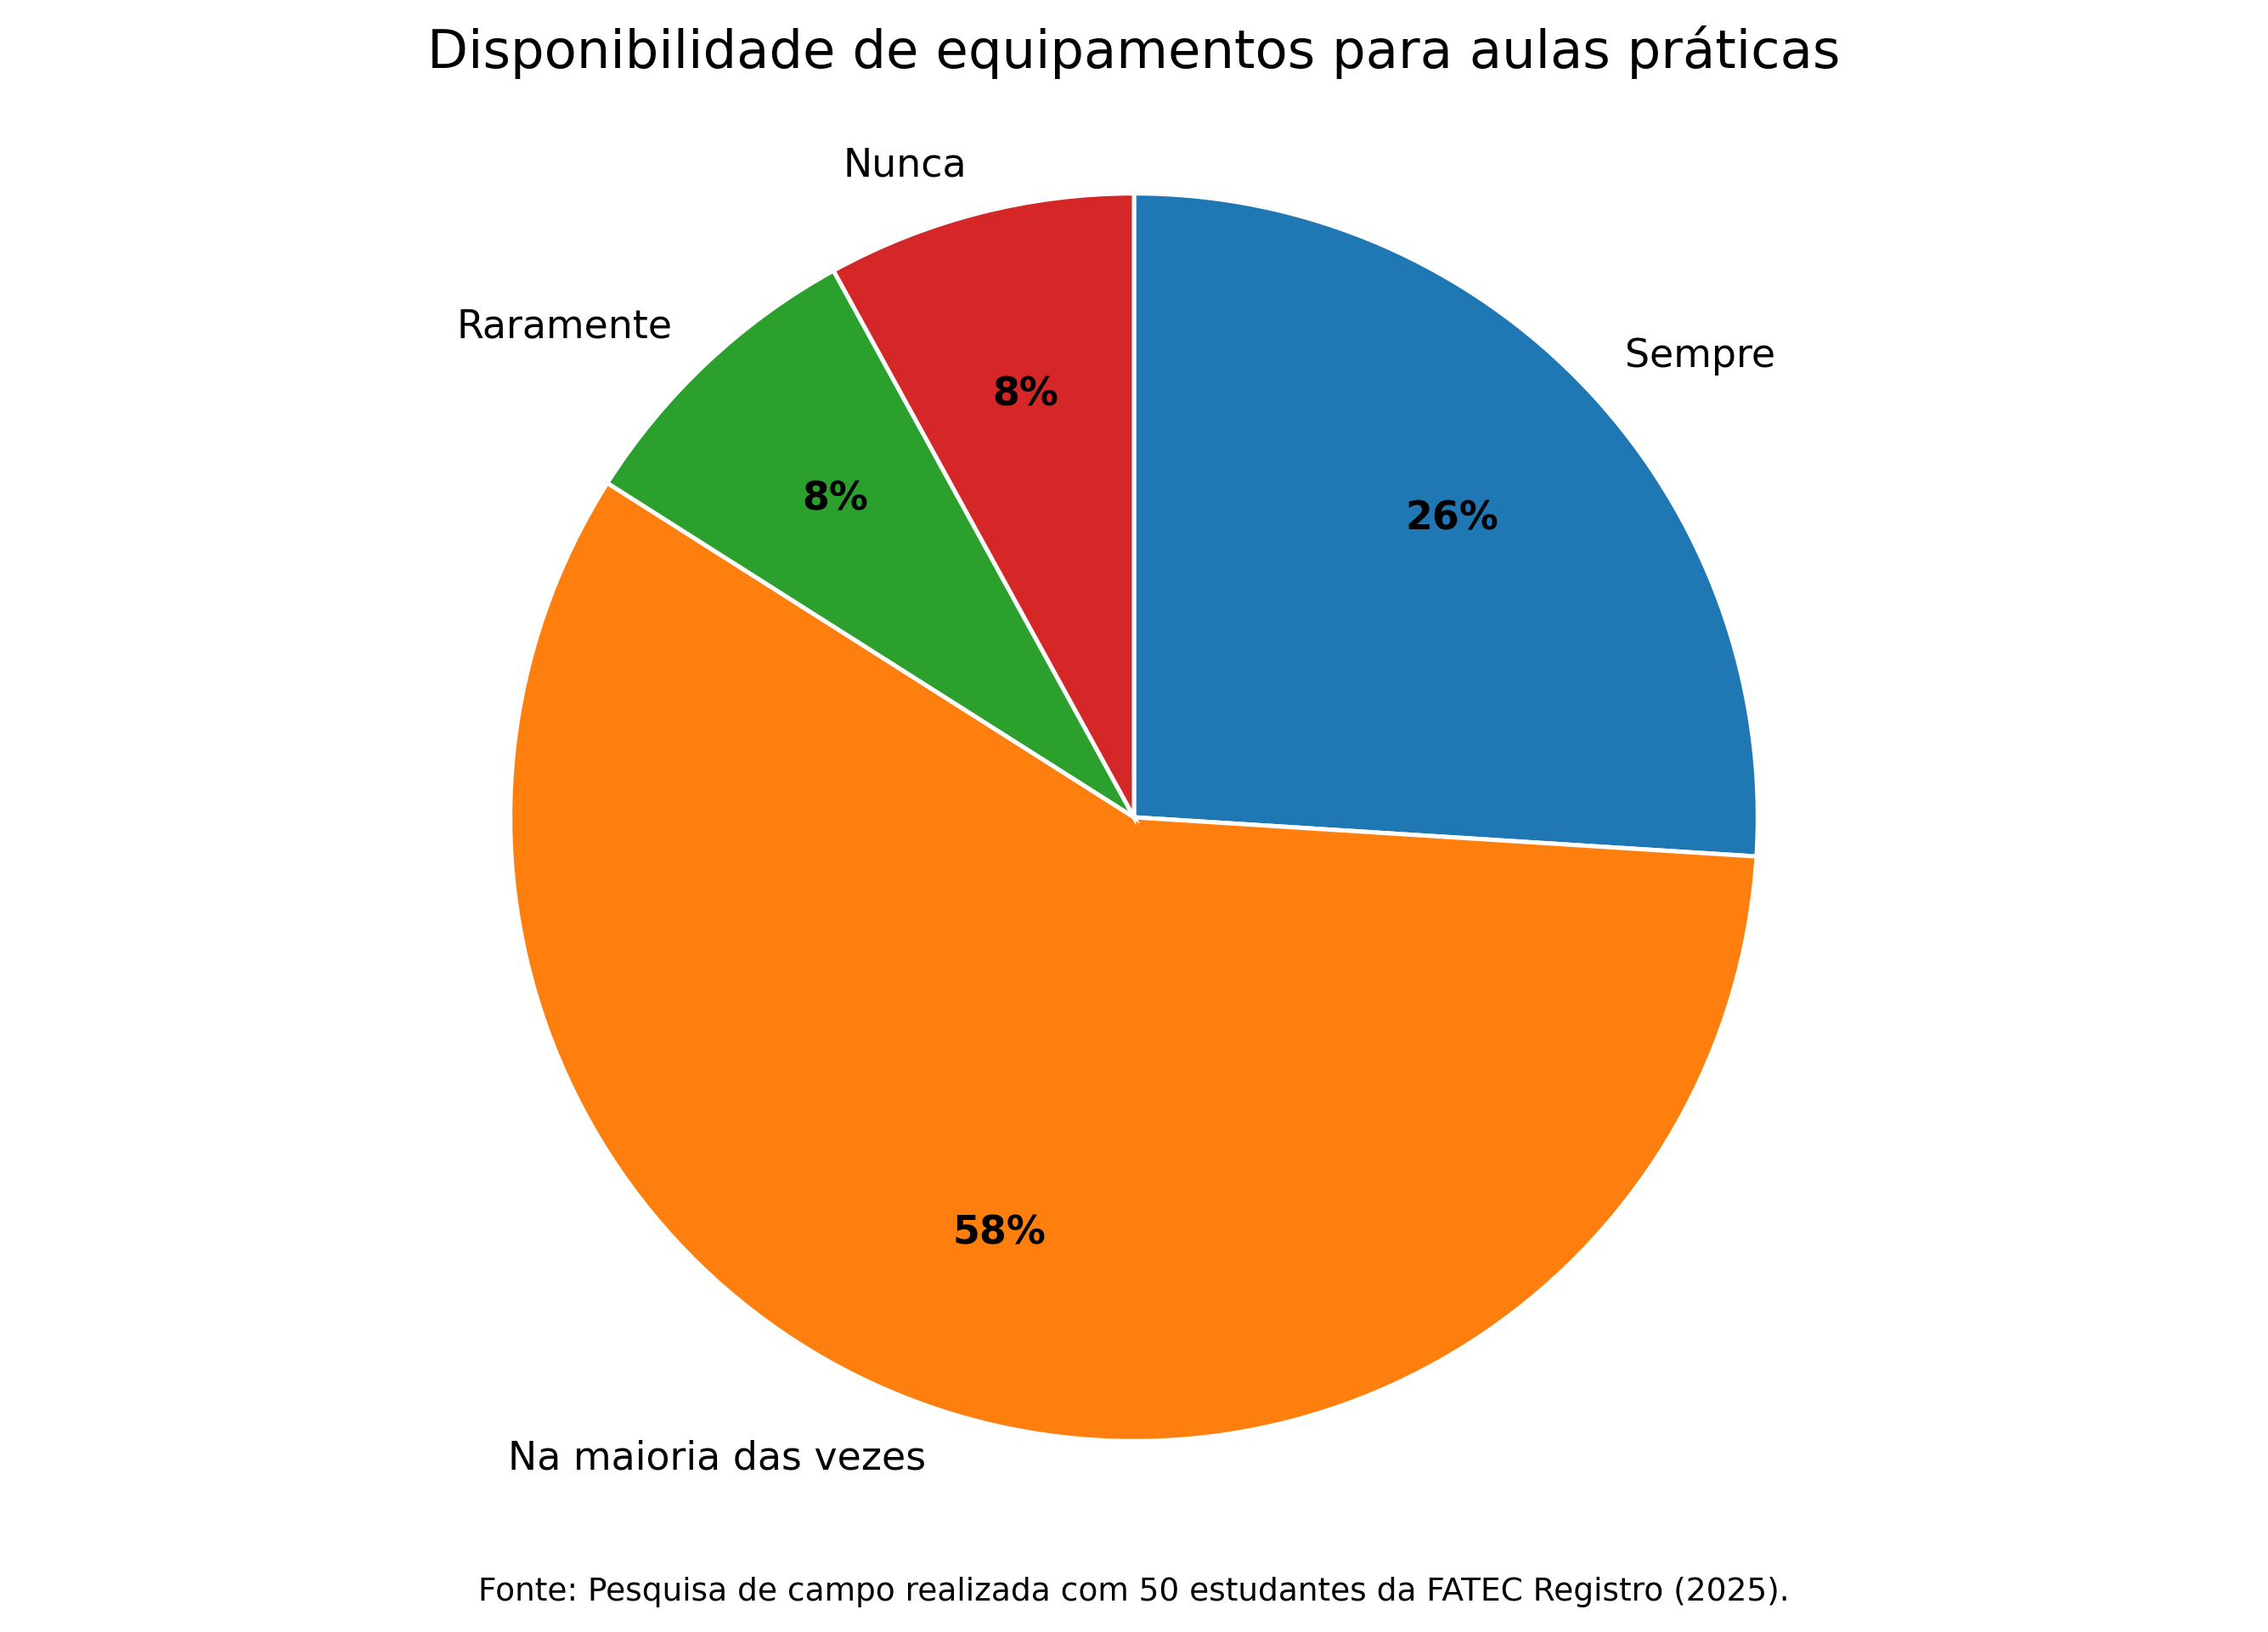
\includegraphics[width=0.65\textwidth]{imgs/pesquisa-q2.png}
    \caption{Disponibilidade de equipamentos para aulas práticas}
    \label{fig:pesquisa-q2}
\end{figure}

A análise conjunta das questões 2 e 3 permitiu compreender como essa limitação afeta a realização das atividades práticas. Entre os estudantes que relataram indisponibilidade de equipamentos, 43,6\% apontaram o revezamento de recursos como principal alternativa, enquanto 30,8\% mencionaram o uso de simuladores. Também foram relatadas a substituição das práticas por materiais teóricos, o uso de equipamentos emprestados e, em menor proporção, a ausência da atividade prática. Esses resultados indicam que, mesmo quando a aula é realizada, a disponibilidade limitada pode exigir estratégias alternativas para viabilizar a participação dos estudantes.

Em relação à adoção de tecnologias acessíveis, a Figura \ref{fig:pesquisa-q9} demonstra que 71,1\% dos participantes consideraram que soluções baseadas em Realidade Aumentada ou Realidade Virtual poderiam contribuir para reduzir as dificuldades decorrentes da falta de equipamentos físicos, enquanto 26,7\% responderam ``talvez'' e 2,2\% responderam negativamente.

\begin{figure}[H]
    \centering
    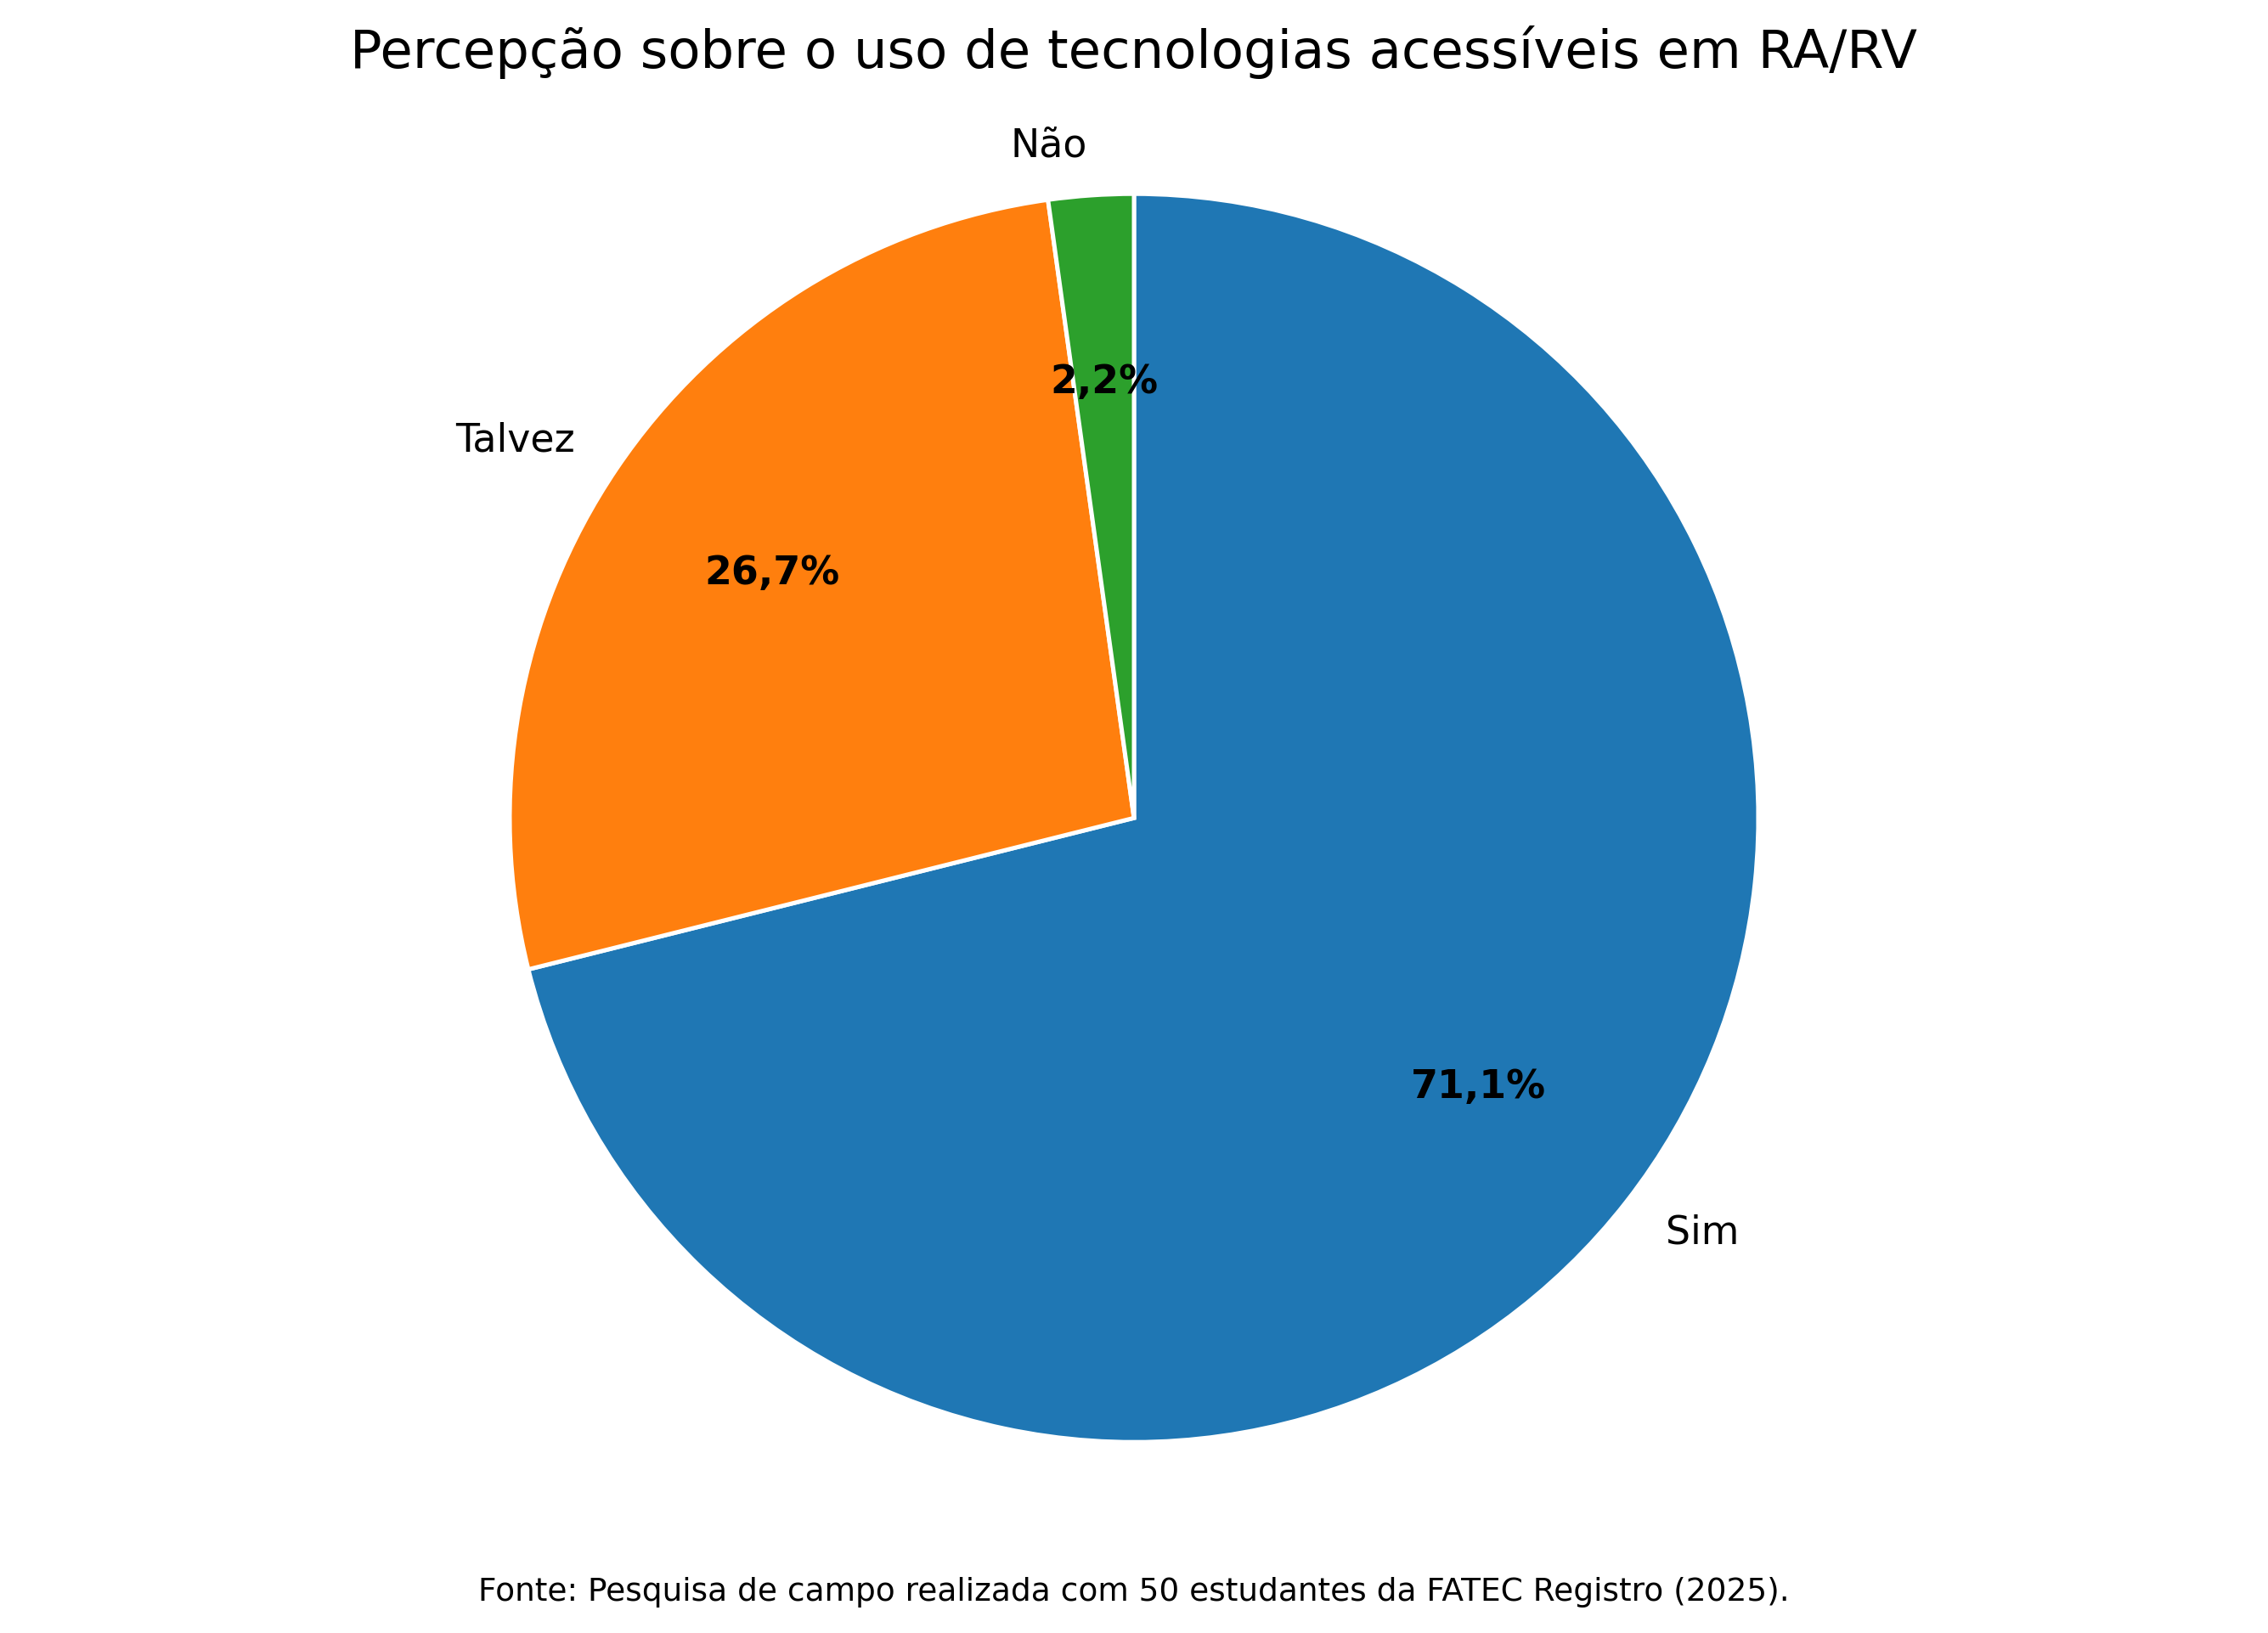
\includegraphics[width=0.65\textwidth]{imgs/pesquisa-q9.png}
    \caption{Percepção sobre o uso de tecnologias acessíveis em RA/RV}
    \label{fig:pesquisa-q9}
\end{figure}

Quanto ao desenvolvimento do protótipo, os testes funcionais e qualitativos demonstraram o funcionamento da detecção de superfícies em Realidade Aumentada, do posicionamento dos componentes tridimensionais e do reconhecimento de gestos para interação com as peças. A integração entre Unity, MediaPipe e Python possibilitou a manipulação dos objetos virtuais por meio dos movimentos da mão, enquanto a comunicação HTTP permitiu a troca de informações necessária durante a interação.

Apesar dos resultados técnicos obtidos, o protótipo ainda apresenta limitações relacionadas à precisão dos movimentos, ao processo de encaixe das peças e à estabilidade da aplicação em dispositivos móveis. Além disso, não foram realizadas medições quantitativas de desempenho nem avaliações experimentais de aprendizagem com estudantes. Dessa forma, os resultados obtidos demonstram a viabilidade técnica do protótipo, mas não permitem, nesta etapa, afirmar sua eficácia pedagógica.

% Conclusão
\section{Conclusão}

\lipsum[18] Com base nos resultados obtidos, conclui-se que a metodologia desenvolvida apresenta excelente desempenho para análise de sistemas complexos. As principais contribuições deste trabalho incluem:

\begin{itemize}
    \item Desenvolvimento de um framework computacional robusto;
    \item Validação experimental dos modelos propostos;
    \item Comparação sistemática com métodos existentes;
    \item Identificação de limitações e oportunidades de melhoria.
\end{itemize}

Trabalhos futuros incluem a extensão da metodologia para sistemas multidimensionais e a incorporação de técnicas de otimização avançadas.

% Agradecimentos
\section*{Agradecimentos}

Os autores agradecem à Faculdade de Tecnologia do Estado de São Paulo (FATEC) e ao Centro Paula Souza (CPS) pelo apoio institucional. Este trabalho foi parcialmente financiado pela FAPESP (proc. 2024/12345-6) e CNPq (proc. 301234/2024-0).

% Referências
\bibliographystyle{IEEEtran}
\bibliography{referencias}

\end{document}
